\section{Convex Hull}\label{sec:ch}
A commonly used compactness score is the \textit{convex hull
score}.  We briefly recall the definition of a convex set and then
define this score function.

\begin{definition}
  Let $\mathrm{conv}(\Omega)$ denote the \textit{convex hull} of
  a region $\Omega$ in either the sphere or the plane, which is the
  smallest convex region containing $\Omega$.  Then we define the
  \textit{convex hull score} of $\Omega$ as 
  \begin{align*}
    \mathrm{CH}(\Omega)=
    \frac{\mathrm{area}(\Omega)}{\mathrm{area}(\mathrm{conv}(\Omega))}
  \end{align*}
\end{definition}
\cut{
The convex hull score of a region $\Omega$  will be equal to one if
and only if $\Omega$ is itself convex.  We note that the convex hull
and Polsby-Popper scores agree when $\Omega$ is a circle, provide
a similar score when $\Omega$ is roughly circluar, and differ greatly
if $\Omega$ is a highly non-circular but convex region, such as
a long, thin rectangle.}

To demonstrate that any map projection cannot preserve
the orders of convex hull scores we note that  
order-preserving map must, in particular, preserve the 
maximizers in the ordering. This means that convex
regions on the sphere are mapped to convex regions in the plane.

By Theorem~\ref{thm:convex_to_convex}, such a map 
must be the gnomonic projection up to a linear transformaion. 
We first show that the gnomonic projection does not preserve 
convex-hull score orderings on any region of the sphere.

\abn{mute this and write it in later:
This lemma lets us prove our theorem in two steps.  We can first show
that the gnomonic projection does not preserve the ordering of convex
hull scores, then argue that this misordering cannot be corrected by
any affine linear transformation of the plane.  This first part we
will prove by explicitly constructing two regions whose convex hull
scores are permuted under the gnomonic projection, and to facilitate
this construction, we make the following observation:}

We finally have the tools to prove the main result of this section,
which is a direct consequence of the four previous lemmas.

\begin{figure}
	\centering
	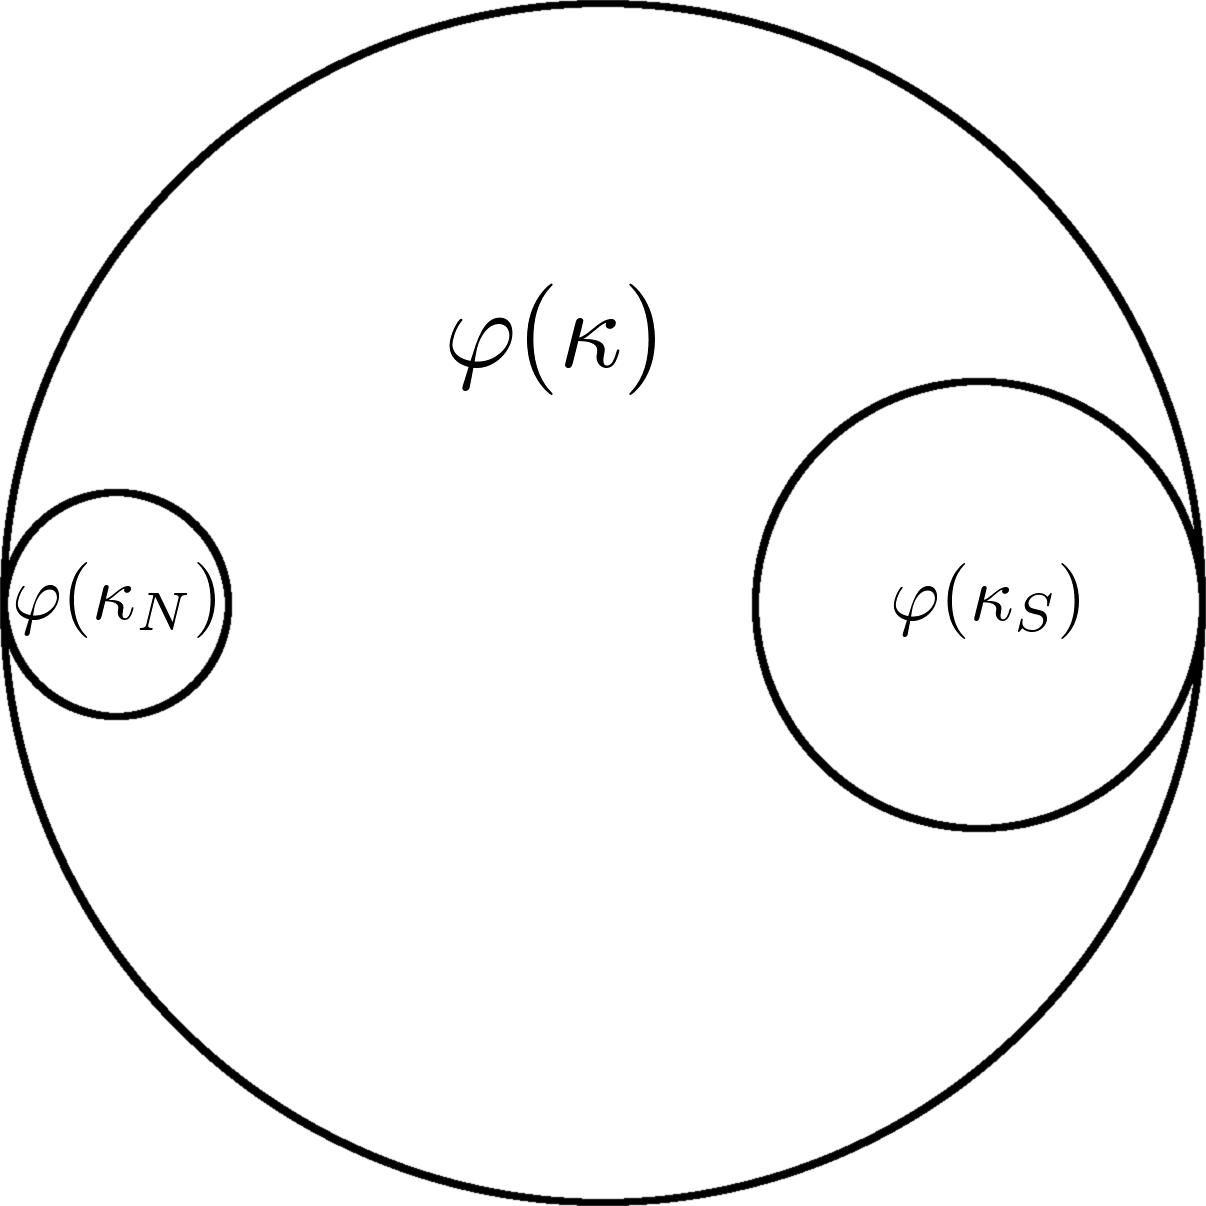
\includegraphics[width=.2\textwidth]{figs/differentkappa}\\[1.5em]
	\caption{ The construction used in \Cref{thm:convhull}. }
	\label{fig:caphr}
\end{figure}

\begin{theorem}
  \label{thm:convhull}
  Let $\Omega$ be a region on the sphere.  Then there exist two regions
  $\kappa'_N,\kappa'_S\subset \Omega$ such that the convex hull scores of
  $\kappa'_N$ and $\kappa'_S$ are equal on the sphere, but under the
  gnomonic projection $\varphi$, the convex hull score of $\kappa'_S$ is
strictly greater than that of $\kappa'_N$.  
\end{theorem}

\begin{proof}
  First, since $\Omega$ is a region, we can find some cap $\kappa$ inside
  of $\Omega$ such that the center of $\kappa$ is not the south pole of the
  sphere, and the north pole is exterior to $\kappa$.  This cap is
  bisected by a line of longitude, in particular the great circle
  which passes through the two poles and the center of $\kappa$.  This
  line of longitude meets $\kappa$ at exactly two points, and we call
  $p_N$ the point closer to the north pole and $p_S$ the point closer
  to the south pole.

  Choose some $r$ strictly less the radius of $\kappa$ and let
  $\kappa'_S$ be the region constructed by deleting a cap of radius
  $r$ from the interior of $\kappa$ tangent at $p_S$.  Construct
  $\kappa'_N$ analogously by deleting a cap of radius $r$ tangent at
  $p_n$. Observe that the convex hull scores of $\kappa'_N$ and
  $\kappa'_S$ are identical, since each has the boundary of $\kappa$
  as its smallest bounding cap and both convex hulls have the same
  area.

  We now consider the images of $\kappa'_N$ and $\kappa'_S$ under the
  gnomonic projection $\varphi$.  Since $\varphi$ preserves points of
  tangency, containment, and sends every cap to an ellipse, the images
  $\varphi(\kappa'_N)$ and $\varphi(\kappa'_S)$ are both regions which
  are ellipses with a smaller ellipse, tangent to a point on the
  circumference, deleted.  Furthermore, since the boundary of $\kappa$
  was the smallest bounding cap of both regions on the sphere, the
  image of the boundary of $\kappa$ under $\varphi$ is the smallest
  bounding circle of the images of these regions in the plane.

  We can now observe that these two regions in the plane do not have
  the same convex hull score.  Both have the same bounding ellipse,
  which is their convex hulls, but $\varphi(\kappa'_N)$ is strictly
  smaller than $\varphi(\kappa'_S)$.  This is because the gnomonic
  projection distorts areas in a way such that regions further from
  the south pole have their areas magnified more than the same region
  closer to the south pole.  If the regions in question are
  sufficiently small, letting $\theta$ denote the polar angle at which
  we consider a small cap on the sphere, a cap of radius $r$ will be
  sent to an ellipse with a major axis (along the line through the
  center of the ellipse and the origin) of length roughly
  $r/\sin^2{\theta}$\zs{check  this}, and a minor axis of length
  $r/\sin{\theta}$, and a straightforward examination of this as
  a function of $\theta$ shows that it grows faster as $\theta$
  increases.

  Since $\varphi(\kappa'_N)$ fills a smaller fraction of the bounding
  ellipse than $\varphi(\kappa'_N)$ does, its convex hull score is
  strictly worse, and the gnomonic projection does not preserve convex
  hull scores.
\end{proof}

Now that we've shown that the gnomonic projection alone cannot
preserve convex hull scores, to complete the argument, we must now
show that there is no affine linear transformation of the plane which
can correct for this.

\begin{lemma}\label{lem:noafflin}
  Let $L$ be an affine linear transformation of the plane.  Then $L$
  preserves the convex hull scores of all figures in the plane.
\end{lemma}
\begin{proof}
  Since affine linear transformations map lines to lines, they preserve
  convexity, and since they also preserve the containment of regions in
  other regions, if $\Omega$ is a region in the plane, then it must be
  the case that the convex hull of $\Omega$ is mapped to the convex hull
  of $L(\Omega)$ by $L$.  In other words, the image of the convex hull
  of $\Omega$ is the convex hull of the image of $\Omega$.  Finally,
  since affine linear transformations preserve the ratio of the areas of
  any two regions, $L$ must, in particular, preserve the ratio of the
  areas of $\Omega$ and its convex hull, so the convex hull score is
  preserved.
\end{proof}
